\section{Marketing - AE}
\label{section_marketing}
Das Marketing hat neben dem typischen Aufgabenbereich der Außenrepräsentation durch die Besonderheiten einer Hochschule auch einen Aufgabenbereich der Innenrepräsentation. Im folgenden werden diese Bereiche getrennt betrachtet.

\subsection{Externes Hochschulmarketing}
\label{subsection_externes_hochschulemarketing}
Das externe Marketing der Hochschule bezieht sich auf die klassischen Marketingaufgaben, das Produkt und die Marke vorteilhaft darzustellen. Im Falle einer Hochschule ist dies die attraktive Darstellung gegenüber zukünftigen Studierenden, Forschungsinteressierten und Geldgebern.

\subsubsection{Webseite}
Zentrales Element bleibt die Hochschulwebseite, die mit aktuellen, offenen Möglichkeiten von HTML 5, CSS 3 und JavaScript den Funktionsumfang einer App erreichen kann, ohne auf spezielle oder spezifische Spezialtechnologien zu setzen. Besonders sei an dieser Stelle die Möglichkeit genannt, mittels Media Queries in CSS Größen und Darstellungsmöglichkeiten von Endgeräten unabhängig von konkreten Betriebssystemen und Hardwareplattformen abzudecken.\footnote{vgl. \cite{w3c_media_queries_url}}

Dies ist vor dem Hintergrund wichtig, dass beispielsweise eine native App für iPhones zwingend durch den Appstore der Firma Apple installiert werden muss\footnote{vgl. \cite{apple_app_distribution_guide_url}}, dessen Nutzungsbedingungen sich für die Hochschule in Form von Kosten oder Inhaltseinschränkungen zu Ungunsten der Hochschule verändern könnten. Mit einer nativen App lässt sich trotzdem nur ein beschränkter Nutzerkreis ansprechen, da mehrere Betriebssysteme und Versionen verbreitet sind.\footnote{vgl. \cite{kantarworldpanel_mobile_betriebssysteme_url}} Sollen mehrere Apps für verschiedene Plattformen gepflegt werden, so ist dies mit zusätzlichen Aufwand, und damit Bindung von Ressourcen verbunden.

Eine Neuauflage der Hochschulwebseite mit aktuellen Möglichkeiten und per CSS an verschiedene Darstellungsgrößen angepasst erreicht dagegen jedes internetfähige Gerät mit Browser. Sollte ein neuer Formfaktor wichtig werden, zum Beispiel der einer Smartwatch, so lässt sich dies über eine Erweiterung des Stylesheets erreichen, ohne eine komplette Neuentwicklung in Auftrag zu geben.

\subsubsection{Soziale Netzwerke}
Soziale Netzwerke wie facebook oder twitter sind nicht eindeutig zu bewerten. Auftritte auf diesen Plattformen können nicht alleine stehen, da nicht jeder einen Account bei einem sozialen Netzwerk hat, benötigen aber durch ständigen Nutzerkontakt eigenständige Pflege und Aufsicht, was an einer kleinen Hochschule Personal bindet.

Für interne Kommunikation und Daten ist ein kommerzielles soziales Netzwerk nicht geeignet, da AGB und Nutzungsbedingungen des Netzwerks mit deutschen Datenschutz- und Urheberrechtsvorgaben, die für eine deutsche Hochschule gelten, in Konflikt stehen können. Auch hier sind Nutzer zu berücksichtigen, die kein Interesse haben, einen Account bei einem sozialen Netzwerk zu eröffnen.

Als Mittel der externen Darstellung ist die Reichweite sozialer Netzwerke potentiell weltweit, was an sich für eine Hochschule mit stark regionaler Bindung \footnote{vgl. \cite{hsel_leitbild_url}} weniger relvant ist. Dennoch sind in subjektiver Wahrnehmung soziale Netzwerke ein wichtiges Kommunikationsmittel und Informationsquelle der Zielgruppe potentieller Studierender. Inwieweit dies speziell für das Einzugsgebiet der Hochschule Emden/Leer gilt ist unbekannt.

Eine Lösung des Konfliktes zwischen Ressourceneinsatz und unbekannter Relevanz ist die öffentlich zugänglichen Informationen der Webseite auch in sozialen Netzwerken zugänglich zu machen. Optimal ist hier, dass kein oder nur geringer Mehraufwand für die zusätzlichen Kommunikationswege entsteht.

\subsubsection{Verteilte Content-Erzeugung}
Im Kontext einer kleinen Hochschule ist die Personalsituation besonders zu berücksichtigen. Es ist nicht praktisch, dass eine oder mehrere Personen zentralisiert die Redaktion aller zu veröffentlichenden Inhalte übernehmen, da relevante Neuigkeiten an mehreren unterschiedlichen Stellen auftreten, und am besten ohne Umweg veröffentlicht werden. Hierzu eignen sich Content-Management-Systeme, die einen Workflow wie in Abbildung 6.1 realisieren.

\begin{figure}[h!]
	\centering
	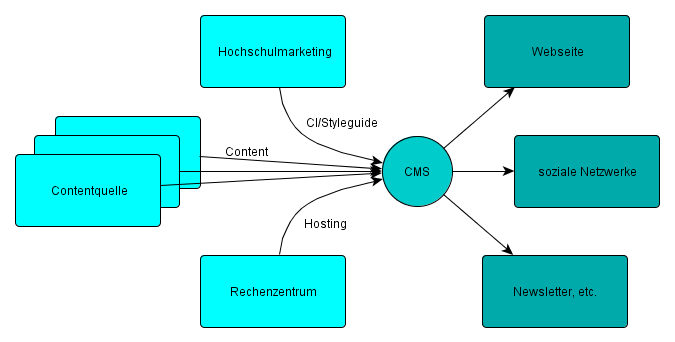
\includegraphics[width=10cm]{kapitel/gruppe3/bilder/verteilter_publishing_workflow}
	\caption{Verteilter Publishing Workflow}
	\label{fig_publishing_workflow}
\end{figure}

Das Hosting wird dabei durch das Rechenzentrum realisiert, während das Hochschulmarketing mit Corporate Identity und Styleguide eine einheitliche Erscheinung der Auftritte leistet. Die Inhalte steuern mehrere, unabhängigen Autoren bei, die mittels unterschiedlicher Berechtigungen und Adressierungen unterschiedliches Publikum erreichen können.
So kann ein unidentifizierter Besucher der Webseite öffentliche, allgemeine Informationen vorfinden, ein angemeldeter Studierender jedoch zusätzlich und prominenter Informationen und Neuigkeiten zu seinem Fachbereich und seinen Kursen.
Weiterhin kann mit einem Content Management System geleistet werden, dass Autoren Inhalte beisteuern und veröffentlichen können, ohne im einzelnen mit den technischen Einzelheiten des Hostings oder des Designs belangt zu werden. Auch können Content Management Systeme Inhalte für weitere Plattformen aufbereiten, zum Beispiel an soziale Netzwerke posten. \footnote{vgl. \cite{content_management_system_patent}}

\subsection{Internes Hochschulmarketing}
\label{subsection_internes_hochschulemarketing}
Im Gegensatz zur Situation in einem Unternehmen genießen einzelne Fachbereiche und Personen in einer Hochschule einen hohen Grad an Freiheit und Autonomie. Daher können in Arbeitsgruppen und Gremien beschlossene Prozesse und Software nicht per Anordnung durchgesetzt werden, sondern müssen nach innen vermarktet werden, um akzeptiert zu werden. Herausfordernd ist hier besonders die Heterogenität, da der technische und fachliche Hintergrund sich unter Mitarbeitern und Fachbereichen erheblich unterscheiden, etwa zwischen technischen und nichttechnischen Fachbereichen.

\subsubsection{Fokussierter Support}
Eine Möglichkeit, Benutzer hin zu einer präferierten Lösung zu leiten ist diese in Präferenzen, Anleitungen und FAQs an erster Stelle und in höherem Detailgrad zu präsentieren. Vielfach wird eine Voreinstellung einfach übernommen, und die erste Lösung zu einer Fragestellung als Referenz angesehen, vergleichbar dem Agenda-Setting.\footnote{vgl. \cite{bonfadelli_medienwirkungsforschung_2015}}

\subsubsection{Schulungen}
Eine weitere Maßnahme ist, Schulungen für die präferierten Lösungen anzubieten, die Vorteile der gefundenen Lösung gegenüber anderen herausstellt. Optimal ist eine solche Lösung transparent, oder aber bietet Alleinstellungsmerkmale, die eine Verwendung aus sich heraus attraktiv erscheinen lassen. Trotzdem kann es vorkommen, dass in Lern- und Umstellungsphasen Lernkurven in der Benutzung absolviert werden müssen. Soll eine Lösung akzeptiert werden, dann muss diese Lernkurve entsprechend begleitet werden.

\subsubsection{Integration}
Eine weitere starke, aber arbeitsintensive Maßnahme ist, die präferierte Lösung stark zu integrieren. Beispielsweise sei die Erstellung von hochwertigen Dokumentvorlagen entsprechend der Corporate Identity für die präferierte Textverarbeitung genannt.

Der Übergang zum fokussierten Support ist hier fließend. Wird die präferierte Lösung an das bestehende System angepasst, so kann von Integration gesprochen werden, wird das System an eine präferierte Lösung angepasst, ist dies fokussierter Support. Beides kann sehr gut gegenseitig ergänzend eingesetzt werden.
